\section{Simulations and data applications}\label{sec:numerical}
This section studies Bayesian-PMALA in simulations and in two data applications. It addresses four questions: how the individual and joint samplers compare with the Laplace and horseshoe Gibbs samplers of \citet{onizuka2024fast} and with the ADMM estimator of \citet{brantley2020baseline} on two benchmark signals, at interior and at extreme quantile levels (Section~\ref{sec:simulations}); how the time per sweep grows with the sample size (Section~\ref{sec:scalability}); how well the method recovers a baseline contaminated by transient peaks (Section~\ref{sec:air_simulation}); and how it performs on an air-quality series and on growth data (Section~\ref{sec:applications}). In every example the order is $k = 2$, and $\lambda$ and $\sigma$ are sampled with the trend. Additional tables and figures are in Appendices~\ref{app:simulation_results} and~\ref{app:data_plots}.

% !TeX root = ../main.tex
\subsection{Simulations on two benchmark signals}
\label{sec:simulations}

We compare Bayesian-PMALA with Bayesian and optimization-based quantile trend filtering on two benchmark signals: the varying-smoothness signal (VS) of \citet{onizuka2024fast}, which adds a localized bump to gradual variation, and the smooth sinusoid (S) of \citet{brantley2020baseline}. Section~\ref{sec:sim:individual} considers interior quantile levels, and Section~\ref{sec:sim:extreme} the joint estimation of extreme upper quantiles. Additional tables are in Appendix~\ref{app:simulation_results}.

For $u_i=i/n$, $i=1,\ldots,n$, and $n=500$, the observations are generated as $y_i=f(u_i)+\varepsilon_i$ with
\begin{align}
 f_{\mathrm{VS}}(u)&=2+\sin(4u-2)+2\exp\{-30(4u-2)^2\},
 \label{eq:sim_vs}\\
 f_{\mathrm{S}}(u)&=\sin(2\pi u).
 \label{eq:sim_s}
\end{align}
The errors follow the three noise families of \citet{onizuka2024fast}. The first is Gaussian, $\varepsilon_i\sim\mathcal{N}(0,s(u_i)^2)$ with $s(u)=(1+u^2)/4$. The second is Beta, $\varepsilon_i\sim\mathrm{Beta}(1,11-10u_i)$. The third is mixed normal, $\varepsilon_i\sim u_i\mathcal{N}(-0.2,0.5)+(1-u_i)\mathcal{N}(0.2,0.5)$, with the component variance as second argument. The target is the true conditional quantile $Q_\tau(u)=f(u)+F_u^{-1}(\tau)$, where $F_u$ is the error distribution at $u$.

\subsubsection{Interior quantiles}
\label{sec:sim:individual}

The competitors are the Laplace and horseshoe Gibbs samplers of \citet{onizuka2024fast} and the ADMM estimator of \citet{brantley2020baseline}. The levels are $\tau=0.05$, $0.25$, $0.50$, $0.75$, and $0.95$, and all methods are fitted to the same data in each replication. Bayesian-PMALA uses $\sigma\sim\mathrm{IG}(0.1,0.1)$. For the VS signal, $\lambda\sim\mathrm{Gamma}(1,10^{-3})$, the interweaving step is used, and the chain has $30000$ sweeps of which the first $10000$ are discarded; for the S signal, $\lambda\sim\mathrm{Gamma}(1,5\times10^{-4})$, no interweaving step is used, and the chain has $20000$ sweeps of which the first $5000$ are discarded. The samplers of \citet{onizuka2024fast} use $8000$ sweeps with $2000$ burn-in and an $\mathrm{IG}(1,1)$ prior on $\sigma^2$. The Bayesian point estimates are posterior means. ADMM selects $\lambda$ by extended BIC over a $25$-point logarithmic grid, and a replication is discarded when any candidate on the grid fails to converge.

For each fit we compute $\mathrm{MSE}=n^{-1}\sum_i(\widehat\theta_{\tau,i}-Q_\tau(u_i))^2$, $\mathrm{MAD}=n^{-1}\sum_i|\widehat\theta_{\tau,i}-Q_\tau(u_i)|$, and, for the samplers, the mean width MCIW of the pointwise $95\%$ intervals. All three are averaged over valid replications.

\label{sec:sim:ind:vs}Table~\ref{tab:vs_int_mse} reports the MSE for the VS signal; MAD and MCIW are in Appendix~\ref{app:sim:individual:vs}. In every configuration the MSE values of the three Bayesian samplers are within a factor of $1.22$ of one another, and the horseshoe has the smallest at all five levels under Beta noise. A single global penalty therefore gives nearly the same error as local shrinkage on this signal. ADMM has the largest MSE in $14$ of the $15$ configurations; the exception is mixed-normal noise at $\tau=0.95$. This is consistent with extended BIC selecting a penalty too large for the localized bump, whereas the samplers estimate a smaller one.

\begin{table}[!htbp]
\centering
\small
\caption{Mean squared error (MSE) for the varying-smoothness (VS) signal ($k=2$), $n=500$, at interior quantile levels.}
\label{tab:vs_int_mse}
\begin{tabular}{lrrrrr}
\toprule
Beta & $0.05$ & $0.25$ & $0.50$ & $0.75$ & $0.95$ \\
\midrule
Onizuka (Laplace) & 0.000513 & 0.001024 & 0.001942 & 0.002994 & 0.007269 \\
Onizuka (Horseshoe) & 0.000512 & 0.000943 & 0.001802 & 0.002778 & 0.006493 \\
Bayesian-PMALA & 0.000541 & 0.001032 & 0.001966 & 0.003035 & 0.007911 \\
ADMM & 0.008055 & 0.004120 & 0.006632 & 0.007613 & 0.014649 \\
\midrule
Mixed normal & $0.05$ & $0.25$ & $0.50$ & $0.75$ & $0.95$ \\
\midrule
Onizuka (Laplace) & 0.075391 & 0.031684 & 0.027303 & 0.031800 & 0.077075 \\
Onizuka (Horseshoe) & 0.073529 & 0.031743 & 0.028090 & 0.033608 & 0.079668 \\
Bayesian-PMALA & 0.081173 & 0.033267 & 0.026919 & 0.031086 & 0.074781 \\
ADMM & 0.096462 & 0.092891 & 0.071678 & 0.049944 & 0.068415 \\
\midrule
Gaussian & $0.05$ & $0.25$ & $0.50$ & $0.75$ & $0.95$ \\
\midrule
Onizuka (Laplace) & 0.020916 & 0.008284 & 0.006932 & 0.007558 & 0.018128 \\
Onizuka (Horseshoe) & 0.019990 & 0.008067 & 0.006651 & 0.007358 & 0.017762 \\
Bayesian-PMALA & 0.019703 & 0.007962 & 0.006803 & 0.007469 & 0.018675 \\
ADMM & 0.088108 & 0.025091 & 0.020181 & 0.014800 & 0.022334 \\
\bottomrule
\end{tabular}
\end{table}

\label{sec:sim:ind:smooth}Table~\ref{tab:s_int_mse} reports the MSE for the S signal; MAD and MCIW are in Appendix~\ref{app:sim:individual:smooth}. ADMM has the smallest MSE in every configuration; the MSE of Bayesian-PMALA is between $1.4$ and $3.1$ times as large. This is the smooth-baseline setting for which ADMM was developed. Bayesian-PMALA has a smaller MSE than both samplers of \citet{onizuka2024fast} at $\tau=0.25$, $0.50$, and $0.75$ under every noise family, by $15\%$ to $23\%$ relative to the better of the two. At $\tau=0.05$ and $0.95$ its MSE is larger than both in five of the six configurations, by $8\%$ to $18\%$ relative to the better of the two; the exception is Beta noise at $\tau=0.05$. This signal has no localized feature to which local shrinkage scales could adapt.

\begin{table}[!htbp]
\centering
\small
\caption{Mean squared error (MSE) for the smooth (S) signal ($k=2$), $n=500$, at interior quantile levels.}
\label{tab:s_int_mse}
\begin{tabular}{lrrrrr}
\toprule
Beta & $0.05$ & $0.25$ & $0.50$ & $0.75$ & $0.95$ \\
\midrule
Onizuka (Laplace) & 0.000295 & 0.000794 & 0.001592 & 0.002311 & 0.005225 \\
Onizuka (Horseshoe) & 0.000423 & 0.000812 & 0.001554 & 0.002270 & 0.005342 \\
Bayesian-PMALA & 0.000251 & 0.000649 & 0.001255 & 0.001832 & 0.006169 \\
ADMM & 0.000183 & 0.000425 & 0.000789 & 0.001078 & 0.002464 \\
\midrule
Mixed normal & $0.05$ & $0.25$ & $0.50$ & $0.75$ & $0.95$ \\
\midrule
Onizuka (Laplace) & 0.071456 & 0.026312 & 0.021974 & 0.027079 & 0.067077 \\
Onizuka (Horseshoe) & 0.074248 & 0.026449 & 0.021783 & 0.027401 & 0.072335 \\
Bayesian-PMALA & 0.079543 & 0.022323 & 0.017629 & 0.021790 & 0.072843 \\
ADMM & 0.030277 & 0.010993 & 0.008228 & 0.010769 & 0.023342 \\
\midrule
Gaussian & $0.05$ & $0.25$ & $0.50$ & $0.75$ & $0.95$ \\
\midrule
Onizuka (Laplace) & 0.014933 & 0.006463 & 0.005581 & 0.006136 & 0.014457 \\
Onizuka (Horseshoe) & 0.016242 & 0.006414 & 0.005364 & 0.006003 & 0.014982 \\
Bayesian-PMALA & 0.016324 & 0.005068 & 0.004114 & 0.004793 & 0.015674 \\
ADMM & 0.006561 & 0.003129 & 0.002456 & 0.002843 & 0.005929 \\
\bottomrule
\end{tabular}
\end{table}

\subsubsection{Joint estimation of extreme upper quantiles}
\label{sec:sim:extreme}

The joint sampler of Section~\ref{subsec:joint} fits $\tau\in\{0.90,0.93,0.96,0.97,0.98,0.99\}$ together. The individual sampler, the two samplers of \citet{onizuka2024fast}, and ADMM are fitted one level at a time to the same data. Tables~\ref{tab:vs_ext_upper_mse} and \ref{tab:s_ext_upper_mse} report the MSE at all six levels, and Appendix~\ref{app:sim:joint_extreme} counts crossings among the four levels from $0.96$ to $0.99$.

On the VS signal the joint sampler has the smallest MSE under Gaussian and mixed-normal noise at every level from $0.93$ upward, and its advantage grows as $\tau$ approaches one: at $\tau=0.99$ under mixed-normal noise its MSE is $0.1240$, against $0.2123$ for the horseshoe sampler and $0.2980$ for ADMM. At $\tau=0.90$ under these two noise families the samplers of \citet{onizuka2024fast} have the smaller MSE. Under Beta noise the horseshoe sampler has the smallest MSE from $\tau=0.90$ to $0.98$, as at interior levels, and at $\tau=0.99$ the joint sampler and the individual sampler have the smallest MSE, both at $0.0132$.

On the S signal ADMM has the smallest MSE under Beta and Gaussian noise, with the joint sampler second. Under mixed-normal noise the ADMM error grows from $0.0158$ at $\tau=0.90$ to $0.2911$ at $\tau=0.99$, whereas that of the joint sampler grows from $0.0280$ to $0.0940$; the joint sampler has the smallest MSE from $\tau=0.97$ upward.

On both signals the joint sampler has a smaller MSE than the individual sampler in every configuration but two, both for the VS signal: with Gaussian noise at $\tau=0.90$ the two values are $0.0135$ and $0.0134$, and with Beta noise at $\tau=0.99$ both are $0.0132$. The posterior means of the joint sampler never cross, whereas every individually fitted method produces crossing curves at these closely spaced levels.

\begin{table}[!htbp]
\centering
\small
\caption{Mean squared error at extreme upper quantiles for the VS signal, $n=500$ and $k=2$. The joint sampler fits the six levels together; the other methods fit each level separately.}
\label{tab:vs_ext_upper_mse}
\begin{tabular}{lrrrrrr}
\toprule
Beta & $0.90$ & $0.93$ & $0.96$ & $0.97$ & $0.98$ & $0.99$ \\
\midrule
Onizuka (Laplace) & 0.0048 & 0.0058 & 0.0087 & 0.0102 & 0.0120 & 0.0156 \\
Onizuka (Horseshoe) & 0.0044 & 0.0054 & 0.0075 & 0.0088 & 0.0104 & 0.0138 \\
Bayesian-PMALA & 0.0055 & 0.0068 & 0.0106 & 0.0124 & 0.0154 & 0.0132 \\
ADMM & 0.0174 & 0.0160 & 0.0169 & 0.0174 & 0.0199 & 0.0183 \\
Joint sampler (non-crossing) & 0.0052 & 0.0057 & 0.0083 & 0.0113 & 0.0126 & 0.0132 \\
\midrule
Mixed normal & $0.90$ & $0.93$ & $0.96$ & $0.97$ & $0.98$ & $0.99$ \\
\midrule
Onizuka (Laplace) & 0.0445 & 0.0562 & 0.0992 & 0.1313 & 0.1692 & 0.2437 \\
Onizuka (Horseshoe) & 0.0497 & 0.0627 & 0.0940 & 0.1183 & 0.1441 & 0.2123 \\
Bayesian-PMALA & 0.0541 & 0.0716 & 0.1203 & 0.1468 & 0.1840 & 0.2458 \\
ADMM & 0.0508 & 0.0570 & 0.0926 & 0.1244 & 0.1845 & 0.2980 \\
Joint sampler (non-crossing) & 0.0520 & 0.0548 & 0.0760 & 0.0880 & 0.1034 & 0.1240 \\
\midrule
Gaussian & $0.90$ & $0.93$ & $0.96$ & $0.97$ & $0.98$ & $0.99$ \\
\midrule
Onizuka (Laplace) & 0.0116 & 0.0144 & 0.0225 & 0.0285 & 0.0350 & 0.0500 \\
Onizuka (Horseshoe) & 0.0116 & 0.0142 & 0.0212 & 0.0259 & 0.0318 & 0.0453 \\
Bayesian-PMALA & 0.0134 & 0.0167 & 0.0271 & 0.0328 & 0.0410 & 0.0502 \\
ADMM & 0.0211 & 0.0224 & 0.0234 & 0.0265 & 0.0321 & 0.0407 \\
Joint sampler (non-crossing) & 0.0135 & 0.0141 & 0.0188 & 0.0223 & 0.0265 & 0.0300 \\
\bottomrule
\end{tabular}
\end{table}

\begin{table}[!htbp]
\centering
\small
\caption{Mean squared error at extreme upper quantiles for the S signal, $n=500$ and $k=2$. The joint sampler fits the six levels together; the other methods fit each level separately.}
\label{tab:s_ext_upper_mse}
\begin{tabular}{lrrrrrr}
\toprule
Beta & $0.90$ & $0.93$ & $0.96$ & $0.97$ & $0.98$ & $0.99$ \\
\midrule
Onizuka (Laplace) & 0.0036 & 0.0043 & 0.0061 & 0.0079 & 0.0097 & 0.0122 \\
Onizuka (Horseshoe) & 0.0037 & 0.0045 & 0.0062 & 0.0075 & 0.0091 & 0.0119 \\
Bayesian-PMALA & 0.0042 & 0.0054 & 0.0088 & 0.0107 & 0.0134 & 0.0121 \\
ADMM & 0.0022 & 0.0025 & 0.0032 & 0.0033 & 0.0039 & 0.0050 \\
Joint sampler (non-crossing) & 0.0029 & 0.0030 & 0.0038 & 0.0041 & 0.0049 & 0.0068 \\
\midrule
Mixed normal & $0.90$ & $0.93$ & $0.96$ & $0.97$ & $0.98$ & $0.99$ \\
\midrule
Onizuka (Laplace) & 0.0392 & 0.0491 & 0.0906 & 0.1254 & 0.1657 & 0.2409 \\
Onizuka (Horseshoe) & 0.0433 & 0.0554 & 0.0860 & 0.1102 & 0.1389 & 0.2003 \\
Bayesian-PMALA & 0.0485 & 0.0629 & 0.1119 & 0.1420 & 0.1765 & 0.2324 \\
ADMM & 0.0158 & 0.0182 & 0.0346 & 0.0714 & 0.1732 & 0.2911 \\
Joint sampler (non-crossing) & 0.0280 & 0.0301 & 0.0430 & 0.0512 & 0.0643 & 0.0940 \\
\midrule
Gaussian & $0.90$ & $0.93$ & $0.96$ & $0.97$ & $0.98$ & $0.99$ \\
\midrule
Onizuka (Laplace) & 0.0092 & 0.0112 & 0.0177 & 0.0239 & 0.0317 & 0.0435 \\
Onizuka (Horseshoe) & 0.0096 & 0.0119 & 0.0178 & 0.0229 & 0.0285 & 0.0406 \\
Bayesian-PMALA & 0.0110 & 0.0143 & 0.0238 & 0.0293 & 0.0378 & 0.0460 \\
ADMM & 0.0045 & 0.0054 & 0.0071 & 0.0086 & 0.0111 & 0.0216 \\
Joint sampler (non-crossing) & 0.0072 & 0.0079 & 0.0107 & 0.0121 & 0.0150 & 0.0219 \\
\bottomrule
\end{tabular}
\end{table}

% !TeX root = ../main.tex
\section{Computational cost}
\label{sec:scalability}

% ===========================================================================
% Evidence: experiments/scalability/ (timings.csv, table_cost_scaling_body.tex, make_cost_figure.py; rewritten 2026-10-01 for the exact augmented sampler).
%   run_config.R        one (method, n, replicate) per R process, both samplers' own source files with clock reads only
%   run_timing*.sh      sequential drivers;  results/raw/*.rds, results/timing_log.txt
%   profile_mvrnorm.R   dense operations of the Onizuka theta draw in isolation -> results/mvrnorm_profile.csv
%   collect.R, analyze.py -> results/numbers.json, results/table_time_body.tex, figures/scal_*.pdf (copied to figures/)
% Every number below is taken from results/numbers.json, table_time_body.tex or mvrnorm_profile.csv.
% 2026-10-02: wall-time-per-run material removed; the section reports time per sweep and its breakdown only.
% Previous versions of this section: notes/scalability_rewrite_20261001/before/scalability.tex.
% ===========================================================================

We compare the time per Gibbs sweep of Bayesian-PMALA with that of the Laplace and horseshoe samplers of \citet{onizuka2024fast}. All three use the same augmentation and differ in the trend update. Bayesian-PMALA computes two proximal maps by ADMM with a fixed iteration budget and banded factorizations (Section~\ref{subsec:pmala}), so its sweep costs $O(n)$. The supplied Onizuka code draws the trend from its Gaussian full conditional by forming the dense inverse of the precision matrix and an eigendecomposition (\texttt{MASS::mvrnorm}), whose cost grows cubically in $n$.

\paragraph{Protocol.} We use the VS signal \eqref{eq:sim_vs} with Gaussian noise, $\tau = 0.5$, $k = 2$ and $n$ from $250$ to $4000$, with the same data for all samplers. The Onizuka code is unmodified, with \texttt{sparse = TRUE}, and both samplers are timed by clock reads around their updates. All runs use one laptop core (Intel Core Ultra 7 155U, R~4.4.1, reference BLAS). Warm-up and setup are excluded, and each entry is the median over up to three replicates with distinct data.

\begin{table}[!htbp]
\centering
\footnotesize
\caption{Time per Gibbs sweep in milliseconds: median over replicates, with the range below ($\dagger$: single replicate). Ratios divide the median Onizuka time by the median Bayesian-PMALA time.}
\label{tab:cost_scaling}
\begin{tabular}{rrrrrr}
\toprule
 & \multicolumn{3}{c}{Time per sweep (ms)} & \multicolumn{2}{c}{Ratio to PMALA} \\
\cmidrule(lr){2-4}\cmidrule(lr){5-6}
$n$ & PMALA & Laplace & Horseshoe & Laplace & Horseshoe \\
\midrule
250 & 2.0 & 48.4 & 47.2 & 25 & 24 \\
 & (1.9--2.8) & (42.4--52.6) & (37.7--72.1) & & \\
\addlinespace
500 & 4.2 & 314 & 318 & 75 & 76 \\
 & (3.6--4.9) & (246--401) & (265--329) & & \\
\addlinespace
1\,000 & 9.2 & 3\,650 & 2\,918 & 398 & 318 \\
 & (6.7--12.0) & (1\,840--4\,648) & (2\,183--3\,657) & & \\
\addlinespace
2\,000 & 16.1 & 21\,857 & 32\,543 & 1\,360 & 2\,025 \\
 & (15.7--23.8) & (20\,633--23\,081) & (22\,905--42\,180) & & \\
\addlinespace
4\,000 & 36.6 & 257\,660 & 241\,459 & 7\,035 & 6\,593 \\
 & (26.7--38.1) & $^{\dagger}$ & $^{\dagger}$ & & \\
\bottomrule
\end{tabular}
\end{table}

\begin{figure}[!htbp]
\centering
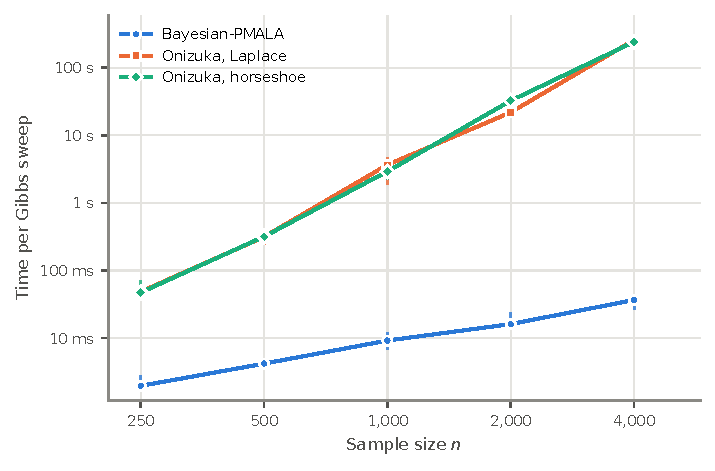
\includegraphics[width=0.7\textwidth]{figures/scal_time.pdf}
\caption{Median time per Gibbs sweep against $n$ (log--log), with bars spanning the range across replicates.}
\label{fig:cost_scaling}
\end{figure}

\paragraph{Results.} The time per sweep of Bayesian-PMALA grows linearly with $n$, at an essentially constant cost per observation, whereas an Onizuka sweep grows roughly cubically, so the gap widens with every doubling of $n$, from about one order of magnitude at the smallest $n$ to nearly four at the largest (Table~\ref{tab:cost_scaling}, Figure~\ref{fig:cost_scaling}). The two Onizuka priors cost the same. Almost all of a Bayesian-PMALA sweep is the P-MALA move, and almost all of an Onizuka sweep is the dense inverse and eigendecomposition of the trend draw (Figure~\ref{fig:cost_breakdown}).

The gap belongs to the supplied implementation rather than to the horseshoe hierarchy, whose precision matrix is banded and admits a banded Cholesky draw. The comparison concerns time per sweep, not the efficiency of the chains per sweep.

\begin{figure}[!htbp]
\centering
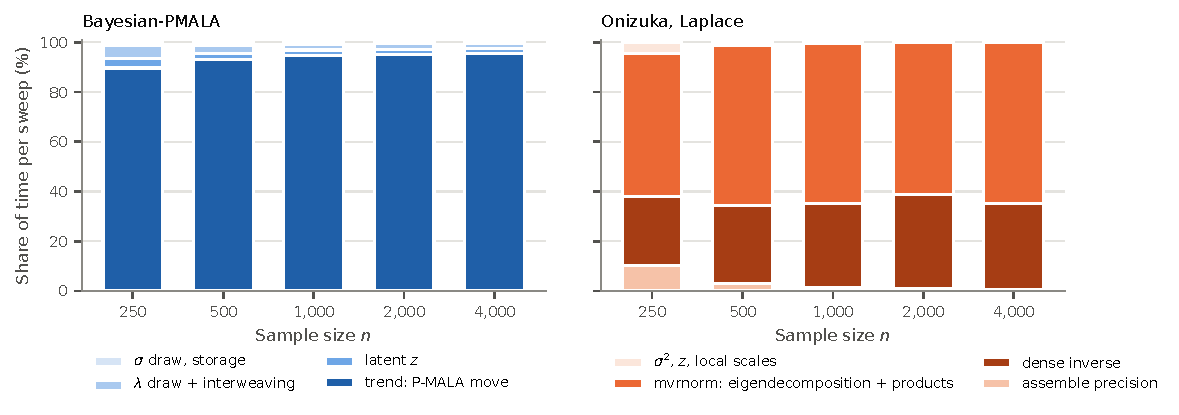
\includegraphics[width=\textwidth]{figures/scal_breakdown.pdf}
\caption{Share of the time per sweep spent in each update (median over replicates). Left: Bayesian-PMALA. Right: the Onizuka Laplace sampler; the horseshoe sampler's shares agree to within three percentage points.}
\label{fig:cost_breakdown}
\end{figure}

% !TeX root = ../main.tex
\subsection{Baseline recovery and peak detection in simulated air-quality data}
\label{sec:air_simulation}

We follow the peak-detection design of \citet[Section~4.2]{brantley2020baseline}, in which a slowly drifting baseline is contaminated by short-lived peaks. The goal is to estimate a low-quantile baseline and to detect the peaks in the detrended series. We compare Bayesian-PMALA with ADMM \citep{brantley2020baseline} and with the Laplace and horseshoe samplers of \citet{onizuka2024fast}, labeled Onizuka (Laplace) and Onizuka (Horseshoe) in Table~\ref{tab:air_n500}.

Each of $100$ replications has $n=500$ equally spaced observations. The baseline $b_i$ is a natural cubic spline with a random number of basis functions and independent $\operatorname{Exp}(1)$ coefficients. A $\operatorname{Binomial}(500,0.005)$ number of Gaussian-shaped peaks is placed at uniformly random locations, with widths drawn from $\operatorname{Unif}(2,12)$ and areas from $\mathcal{N}(20,4^2)$, and $s_i$ is their sum. The observations are $y_i=b_i+s_i+e_i$ with $e_i\stackrel{\mathrm{iid}}{\sim}\mathcal{N}(0,0.25^2)$. At each level $\tau\in\{0.01,0.05,0.10\}$, the estimand is the $\tau$-quantile of the peak-free series, $q_{\tau,i}=b_i+0.25\,\Phi^{-1}(\tau)$. Each method fits every level separately to the same $\by$; $b$ and $s$ are used only for evaluation.

This problem differs in structure from the simulations of Section~\ref{sec:simulations}: the data are a slowly varying baseline plus sparse, one-sided peaks, the working likelihood treats $s_i+e_i$ as the error, and the separation of baseline from peaks is not determined by the data alone, because a short peak can equally be read as a rough stretch of trend. With $a_0=1$, as in Section~\ref{sec:simulations}, the penalty settles where the roughness of the fitted trend puts it (Section~\ref{sec:theory-remarks}), and the fitted baseline bends into the peaks. In this section and in Section~\ref{sec:app:spod} we therefore use $\lambda\sim\mathrm{Gamma}(n,b_0)$: in the full conditional \eqref{eq:lambdaupdate}, $\mathrm{Gamma}(a_0+m,\ b_0+\norm{D\theta}_1)$, the shape $a_0=n$ adds $n$ to $m=n-k-1$ and so roughly doubles $\lambda$ at a given roughness of the trend. This heavier smoothing encodes the assumption that the baseline varies much more slowly than the peaks. In this simulation the fitted roughness $\norm{D\theta}_1$ is of the same order as $b_0$, so the prior and the data contribute about equally to both the shape and the rate of \eqref{eq:lambdaupdate}, and $b_0$ matters; it is chosen by the rule below. On the sensor data of Section~\ref{sec:app:spod} the roughness is much larger than $b_0$, and the posterior median of $\lambda$ changes by at most $12\%$ over the rates tried.

The rate $b_0=10^{-2}$ was chosen on this simulation by a rule fixed before the fits were run, over $b_0\in\{10^{-2},10^{-3},\dots,10^{-6}\}$ at each level, with the three chosen rates differing by at most a factor of ten. The value $b_0=10^{-2}$, the largest of the grid, was the only eligible rate at each level within one paired standard error of the smallest mean MSE, so no further ranking was needed. The sampler is that of the interior simulations (Appendix~\ref{app:pmala:settings}), run for $30{,}000$ sweeps with a burn-in of $10{,}000$, and the fitted curve is the posterior mean.

For a fitted curve $\widehat\theta_\tau$ we report the MSE against $q_\tau$ and the mean check loss (CL) on $\by$. Peaks are detected as the points with $y_i-\widehat\theta_{\tau,i}>h$, for $h\in\{0.5,0.75,1,1.2\}$, and compared with the true signal points $s_i>0.5$ by the class-averaged accuracy (CAA), the mean of sensitivity and specificity. Each metric is averaged over replications; CAA uses the $91$ replications that contain both signal and signal-free points.

\begin{table}[tb]
\centering
\small
\setlength{\tabcolsep}{4pt}
\caption{Simulated air-quality data, $n=500$ and $100$ replications. MSE is measured against the quantile of the peak-free series, CL is the mean check loss, and CAA is the class-averaged accuracy of peak detection at threshold $h$. Entries are means across replications. Bayesian-PMALA uses $\lambda\sim\mathrm{Gamma}(n,10^{-2})$. ADMM is refitted to the same data, the Onizuka (Laplace) entries are computed from archived fits to the same data, and the Onizuka (Horseshoe) entries are carried over unchanged from our original run of this design, whose per-replication results were not retained. $^{\dagger}$Average over $99$ replications ($90$ for CAA).}
\label{tab:air_n500}
\begin{tabular}{@{}rlrrrrrr@{}}
\toprule
 & & & & \multicolumn{4}{c}{CAA at threshold $h$} \\
\cmidrule(lr){5-8}
$\tau$ & Method & MSE & CL & $0.5$ & $0.75$ & $1$ & $1.2$ \\
\midrule
0.01 & Bayesian-PMALA & 0.0232 & 0.00663 & 0.713 & 0.840 & 0.832 & 0.764 \\
0.01 & ADMM & 0.0302 & 0.00642 & 0.687 & 0.818 & 0.838 & 0.780 \\
0.01 & Onizuka (Laplace) & 0.0980 & 0.00508 & 0.633 & 0.664 & 0.642 & 0.613 \\
0.01 & Onizuka (Horseshoe) & 0.0845 & 0.00541 & 0.619 & 0.670 & 0.656 & 0.627 \\
\addlinespace[3pt]
0.05 & Bayesian-PMALA & 0.0143 & 0.02870 & 0.793 & 0.859 & 0.799 & 0.720 \\
0.05 & ADMM$^{\dagger}$ & 0.0127 & 0.02925 & 0.792 & 0.876 & 0.825 & 0.743 \\
0.05 & Onizuka (Laplace) & 0.0848 & 0.02258 & 0.619 & 0.619 & 0.597 & 0.572 \\
0.05 & Onizuka (Horseshoe) & 0.1067 & 0.02354 & 0.579 & 0.580 & 0.556 & 0.534 \\
\addlinespace[3pt]
0.10 & Bayesian-PMALA & 0.0128 & 0.05034 & 0.839 & 0.847 & 0.762 & 0.684 \\
0.10 & ADMM & 0.0114 & 0.05130 & 0.843 & 0.870 & 0.789 & 0.706 \\
0.10 & Onizuka (Laplace) & 0.0651 & 0.04276 & 0.671 & 0.649 & 0.609 & 0.580 \\
0.10 & Onizuka (Horseshoe) & 0.1029 & 0.04166 & 0.572 & 0.551 & 0.533 & 0.517 \\
\bottomrule
\end{tabular}
\end{table}

Bayesian-PMALA and ADMM have comparable MSE at all three levels: $0.0232$, $0.0143$ and $0.0128$ at $\tau=0.01$, $0.05$ and $0.10$ for Bayesian-PMALA in Table~\ref{tab:air_n500}, against $0.0302$, $0.0127$ and $0.0114$ for ADMM. Over the replications common to both methods, the mean difference in MSE, Bayesian-PMALA minus ADMM, is $-0.0070$ (standard error $0.0041$) at $\tau=0.01$, $0.0015$ ($0.0014$) at $\tau=0.05$ and $0.0014$ ($0.0012$) at $\tau=0.10$, each within two standard errors of zero. The other metrics are mixed (Appendix~\ref{app:sim:air}). At $\tau=0.05$ and $0.10$, Bayesian-PMALA has a slightly lower check loss and a lower CAA at the thresholds $h\ge0.75$; at $\tau=0.01$, it has a higher check loss and a higher CAA at $h=0.5$ and $0.75$. The fits of the two samplers of \citet{onizuka2024fast} have the smallest check losses but the largest MSE, between $0.065$ and $0.107$, against at most $0.0302$ for Bayesian-PMALA and ADMM, and their CAA is lower than that of Bayesian-PMALA at every level and threshold. Between their two priors, the Laplace prior has the smaller MSE at $\tau=0.05$ and $0.10$ and the horseshoe at $\tau=0.01$. Small check losses with a large MSE are consistent with fits that follow the peaks rather than the baseline beneath them.

% !TeX root = ../main.tex
\subsection{Data applications}
\label{sec:applications}

We apply the individual sampler of Section~\ref{subsec:individual} to two real data sets, each with a frequentist benchmark. The first is one day of readings from a low-cost air-quality sensor, aggregated to $n = 8{,}640$ observations, where the target is a low quantile of the series that serves as its baseline. The second is the height of 4{,}817 boys and 5{,}190 girls aged 0 to 22 years from the Fifth Dutch Growth Study, where the target is a family of five quantile curves in age.

\subsubsection{Air-quality sensor data}
\label{sec:app:spod}

The first application is the fenceline monitoring problem for which \citet{brantley2020baseline} developed quantile trend filtering. The U.S.\ Environmental Protection Agency places low-cost SPod sensors on the perimeter of industrial facilities to detect fugitive emissions of volatile organic compounds. Each sensor records, once per second, the signal of a photoionization detector (PID) in uncalibrated counts. Emission plumes produce one-sided spikes lasting seconds to a few minutes, on a baseline that drifts over hours with temperature, humidity, and lamp condition. The baseline is therefore a low conditional quantile of the series, and it must be removed before events can be flagged or compared across sensors.

We analyze one day of data, June 15, 2018, from sensor \texttt{d} of the two collocated SPods in the EPA Rubbertown data set accompanying \citet{brantley2020baseline}. The day has $86{,}179$ usable 1-Hz readings; the other seconds are absent or, for $30$ consecutive seconds, recorded as not available. The readings are aggregated into 10-second means of the available readings, so that $n = 8{,}640$ ($19$ of the $8{,}640$ blocks, which contain no reading, are linearly interpolated). The aggregation attenuates the strong serial correlation of the 1-Hz noise, which the ALD working likelihood does not model.

We estimate the baseline at the three levels $\tau \in \{0.01, 0.05, 0.10\}$ with $k = 2$. Each level is fitted separately by the individual sampler on the standardized series, with the sampler and settings of Section~\ref{sec:air_simulation}. The series has the structure of that simulation, short one-sided plumes on a slowly varying baseline, and by the argument given there we use the same prior, $\lambda \sim \mathrm{Gamma}(n, 10^{-2})$ with $n = 8{,}640$. At each level we run two chains of $30{,}000$ sweeps with a burn-in of $10{,}000$, pool every $30$th retained draw of both, and report the pointwise posterior median, transformed back to counts. Under this prior the trend mixes slowly (Appendix~\ref{app:pmala:interior}), so the curves are reported as point estimates, without intervals.

As the frequentist benchmark we use the ADMM solver of the \texttt{detrendr} package of \citet{brantley2020baseline}. Its penalty is selected by extended BIC over the grid $\lambda \in \exp\{-2, \dots, 12\}$. The criterion selects $\lambda = 54.6$ at $\tau = 0.01$ and $\lambda = 1096.6$ at $\tau \in \{0.05, 0.10\}$. Following \citet{brantley2020baseline}, we detect events by a threshold rule on the detrended series $\by - \widehat{\theta}$: a point is classified as signal when it exceeds the empirical 90th, 95th, or 99th percentile of the detrended data. The rule requires no absolute calibration of the counts.

\begin{figure}[tbp]
\centering
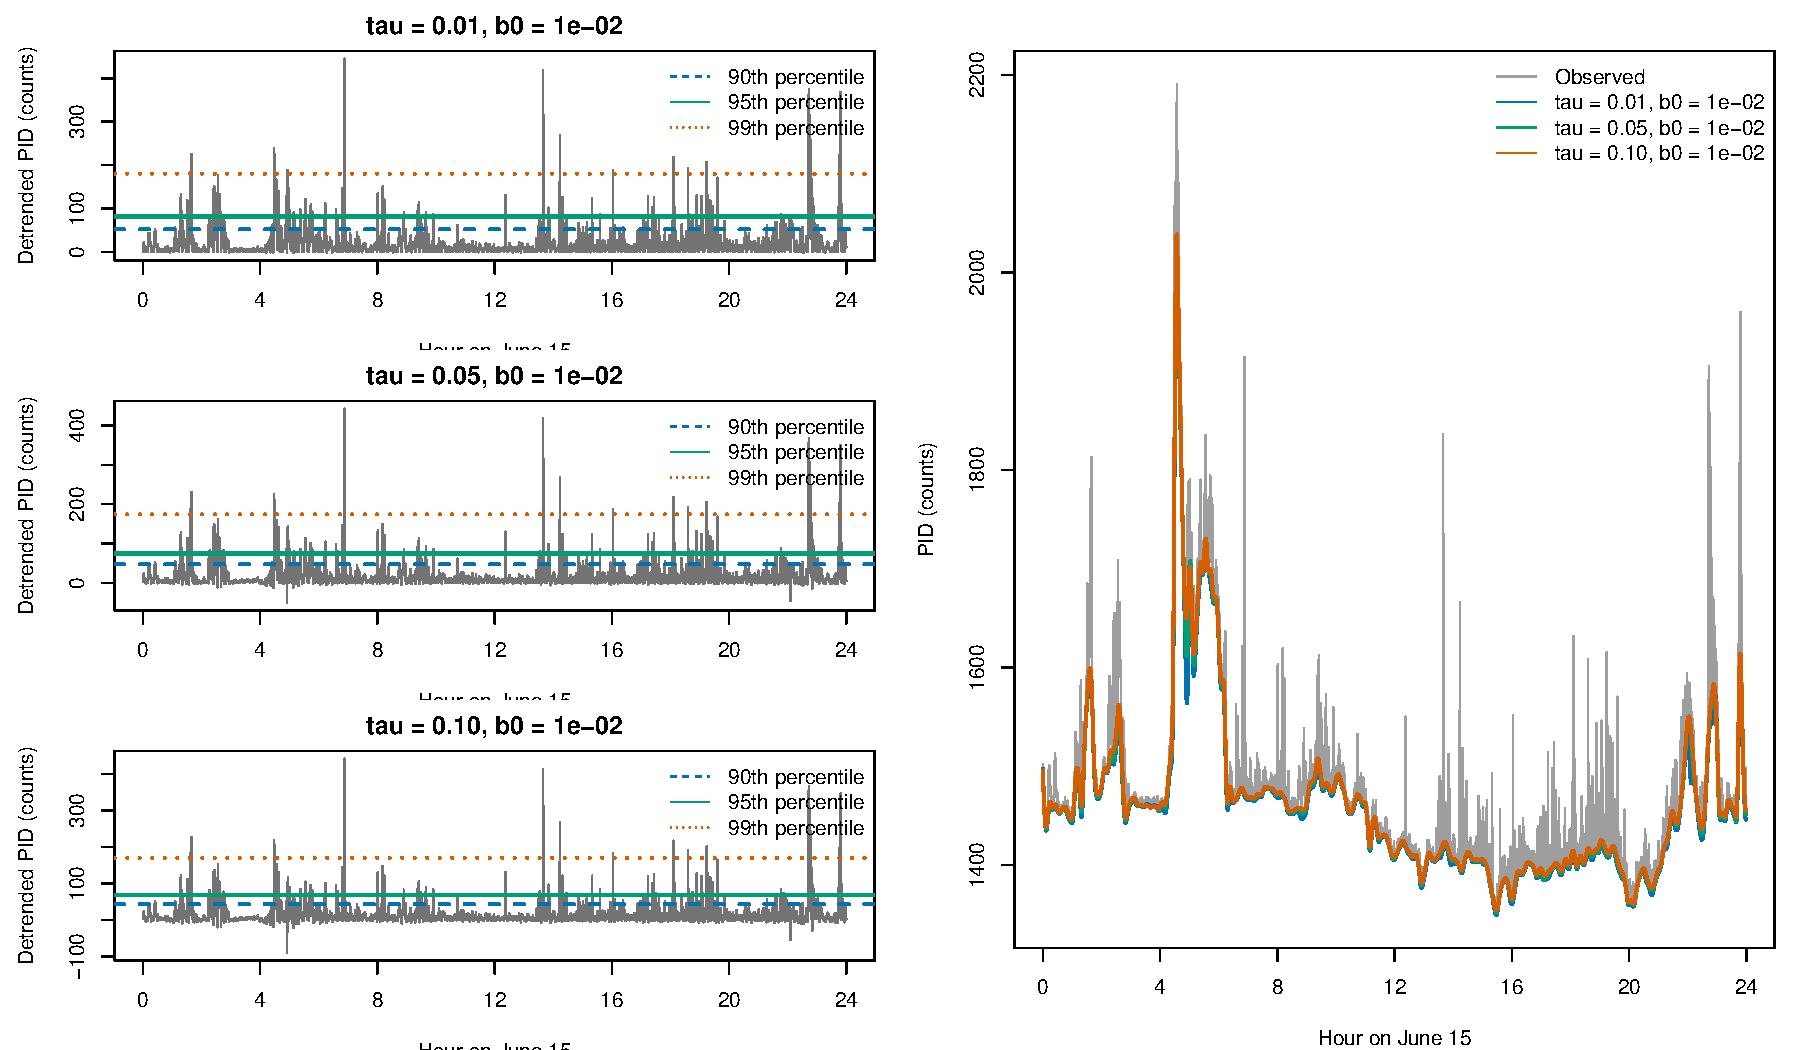
\includegraphics[width=\textwidth]{figures/spod_pmala_e18}
\caption{Air-quality data: Bayesian-PMALA fits with $k = 2$ and $\lambda \sim \mathrm{Gamma}(n, 10^{-2})$ on the 10-second means ($n = 8{,}640$) of SPod \texttt{d}, June 15, 2018. Left: detrended series $\by - \widehat{\theta}$, one panel per quantile level, with the 90th (dashed), 95th (solid), and 99th (dotted) empirical percentiles of the detrended data, the thresholds used to classify emission events. Right: baseline trends at $\tau \in \{0.01, 0.05, 0.10\}$, with the observed PID series in gray. Curves are pointwise posterior medians of two pooled chains.}
\label{fig:spod_pmala}
\end{figure}

The right panel of Figure~\ref{fig:spod_pmala} shows the three fitted baselines for Bayesian-PMALA; the ADMM fits and the detrended series they produce are in Appendix~\ref{app:spod_admm}. Both methods place most of the large excursion between 04:30 and 06:00 in the baseline, follow the slow decline through the afternoon, and leave the short plume spikes above the fit. The fraction of observations below the fitted curve is $0.009$, $0.059$, and $0.116$ at $\tau = 0.01, 0.05, 0.10$ for Bayesian-PMALA, against $0.000$, $0.043$, and $0.092$ for ADMM.

The three levels are fitted separately, so the curves are not constrained to be ordered, and they lie close together: the median distance between adjacent curves is about $1.5$ counts. At $1{,}097$ of the $8{,}640$ time points at least one adjacent pair is in the wrong order (the $0.01$ curve is above the $0.05$ curve at $812$ points, and the $0.05$ curve above the $0.10$ curve at $427$), by at most $6.3$ counts. The ADMM curves also cross: extended BIC selects a penalty twenty times smaller at $\tau = 0.01$ than at the other two levels, and the resulting curve bends upward into the plume near 05:00 and crosses the other two. The joint sampler of Section~\ref{subsec:joint}, which excludes crossings, was not run on these data.

The left panels of Figure~\ref{fig:spod_pmala} show the detrended series with the three detection thresholds, and Figure~\ref{fig:spod_detrended_admm} shows the ADMM counterpart. With the $\tau = 0.05$ baseline removed, the 95\% threshold is $74$ counts for Bayesian-PMALA and $92$ for ADMM, whereas the largest plume exceeds $400$ counts. The events of interest are therefore separated from the noise under either baseline.

Each chain of $30{,}000$ sweeps at $n = 8{,}640$ took between $37$ and $49$ minutes on one core of a Linux compute cluster. The ADMM fit with its grid search took roughly four minutes; it was not timed on the same machine, so the two times are not directly comparable.

\subsubsection{Growth centiles for Dutch children}
\label{sec:app:growth}

The second application is the growth chart: a child's height is read against the population centiles at the same age, so the chart is a family of quantile curves indexed by age. We use the Fifth Dutch Growth Study \citep{schonbeck2013tallest}, a nationwide cross-sectional sample collected in 2009 and distributed with the \texttt{mice} package \citep{vanbuuren2011mice}. After removing records without a height measurement, the data contain 4{,}817 boys and 5{,}190 girls aged 0 to 22 years, each measured once. Boys and girls are analyzed separately.

In contrast with the simulation designs, many children share a covariate value. We round age to the nearest tenth of a year, which gives a grid of $G = 220$ equally spaced ages for boys and $G = 221$ for girls, and index the trend $\theta \in \R^{G}$ by grid point. The ALD likelihood sums the check loss over all children at a grid point, so that each $\theta_g$ is informed by every height recorded at grid point $g$. In the augmented sampler each child keeps its own latent variable $z_i$, and the scale update \eqref{eq:sigmaupdate} runs over all children. In the trend target \eqref{eq:Utheta}, the Gaussian terms of the children at grid point $g$ combine into a single term in $\theta_g$, whose weight is the sum of their $w_i$ and whose center is the $w$-weighted mean of their $r_i$. Because the grid is equally spaced, the difference operator is the usual one, and the samplers apply without other changes.

We use $k = 2$ and $\lambda \sim \mathrm{Gamma}(1, \sqrt{G})$. Each level $\tau \in \{0.1, 0.3, 0.5, 0.7, 0.9\}$ is fitted by an independent run of 6{,}000 sweeps with 1{,}000 burn-in, and we report the posterior mean. This rate differs from those of the simulations, which have one observation per design point, because with some twenty children per grid point the likelihood is much more concentrated.

As a benchmark we fit the LMS method \citep{cole1992smoothing}, the standard tool for growth references. At each age, height is assumed to follow a Box--Cox Cole--Green distribution whose median, coefficient of variation, and Box--Cox power are smooth functions of age. All centiles are read off this one fitted distribution, so they cannot cross; the method assumes a parametric shape at every age. We use the \texttt{lms} function of the \texttt{gamlss} package \citep{rigby2005generalized}.

Figure~\ref{fig:growth_boys} shows the five fitted quantile curves for boys. The curves follow the fast growth in infancy, the near-linear childhood phase, the pubertal spurt, and the adult plateau, and they fan out with age as the height distribution widens. In-sample calibration is close to nominal: the fraction of boys below the fitted curve is $0.098$, $0.300$, $0.498$, $0.699$, and $0.903$ at $\tau = 0.1, 0.3, 0.5, 0.7, 0.9$.

The five fits are independent, so non-crossing is not enforced. The posterior-mean curves for girls do not cross. Those for boys cross in one of $880$ adjacent comparisons: at age $0.1$ years the $0.5$ curve lies $0.6$~cm above the $0.7$ curve.

The girls' fit and the LMS centiles for both sexes are in Appendix~\ref{app:growth} (Figures~\ref{fig:growth_girls}--\ref{fig:growth_lms_girls}). The two methods agree between about one and eighteen years of age and differ at the ends of the age range, where few children are observed. The LMS centiles follow the local data more closely. The trend filtering curves extrapolate the piecewise-quadratic trend: they lie slightly above the newborn measurements and bend at the oldest ages.

\begin{figure}[htbp]
\centering
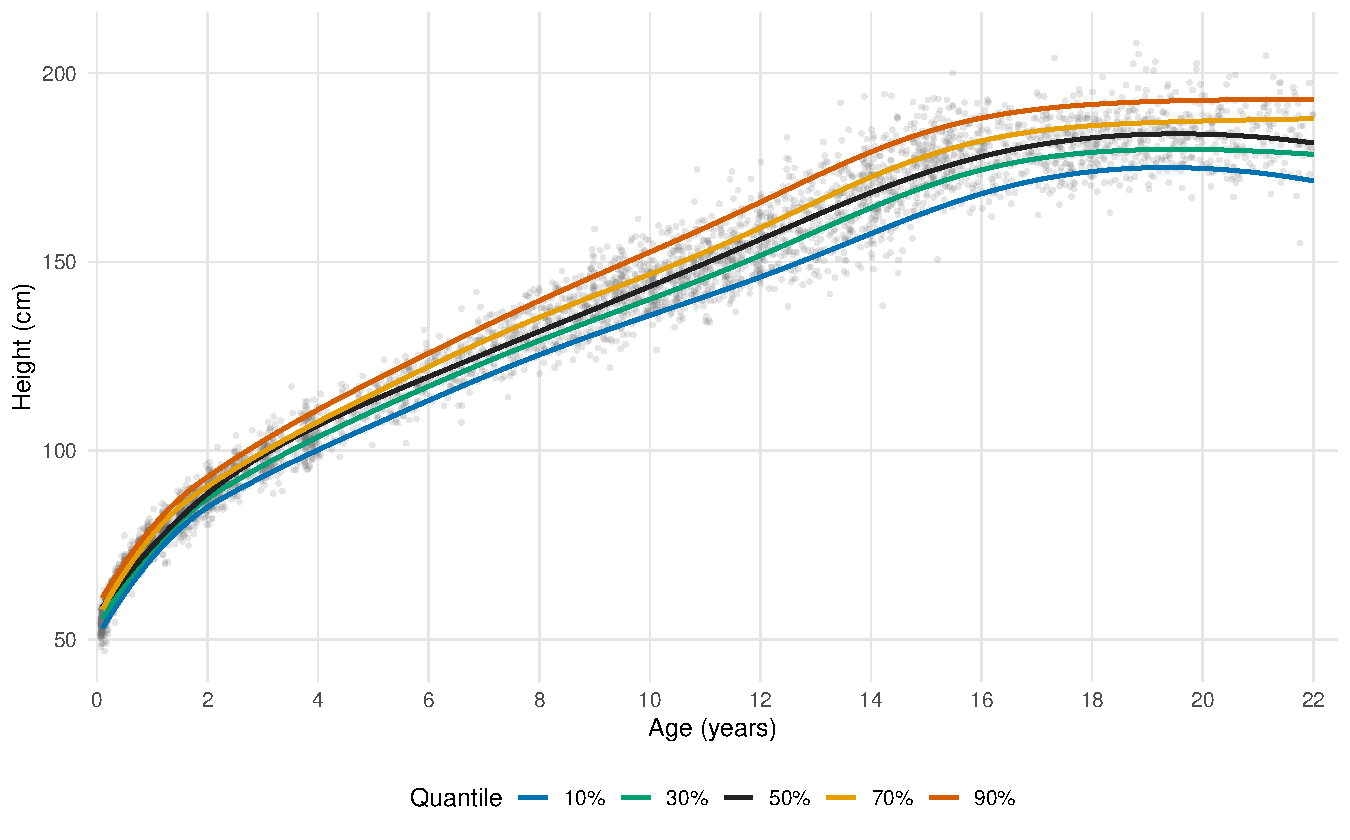
\includegraphics[width=0.75\textwidth]{figures/growth_pmala_boys}
\caption{Bayesian-PMALA fits for the height of 4{,}817 Dutch boys from the Fifth Dutch Growth Study \citep{schonbeck2013tallest} at $\tau \in \{0.1, 0.3, 0.5, 0.7, 0.9\}$, $k = 2$. Curves are posterior means on the 0.1-year age grid; gray circles are the individual measurements. Each level is fitted independently.}
\label{fig:growth_boys}
\end{figure}

